\documentclass[conference]{IEEEtran}
\usepackage{cite}
\usepackage{amsmath,amssymb}
\usepackage{graphicx}
\usepackage{booktabs}
\usepackage{url}
\usepackage[T1]{fontenc}
\usepackage{textcomp}

\begin{document}

\title{Repair or Decline: Checker-Guided LLM Agents for Quality Control of Root Strain-Rate Measurements}

\author{\IEEEauthorblockN{Andrew Oldag}
\IEEEauthorblockA{Division of Biology and Biological Engineering\\
California Institute of Technology\\
Pasadena, CA, USA\\
aoldag@caltech.edu}}

\maketitle

\begin{abstract}
A growing plant root is a slender rod whose material generates its own strain, and its strain-rate field is measured by image correlation on time-lapse movies. The measurement can fail silently through stage drift, low texture, a second root or a jittering midline. We built a system in which deterministic checks derived from beam kinematics test every measurement, an LLM agent names the fault behind a failed check and either repairs the measurement with a remedy from a fixed list or declines to report it, and a second agent audits each root. On 51 held-out synthetic rods with known fields the agent matched a rule-based remedy tree in balanced accuracy and made no false accepts. On compound and novel faults the tree was not written for, the tree was more accurate, because the agent declined repairable rods. An integrated run over 101 real roots and 1,189 windows completed unattended. The checks, not the agent, carried most of the reliability.
\end{abstract}

\begin{IEEEkeywords}
LLM agents, selective prediction, plant growth kinematics, digital image correlation, verification
\end{IEEEkeywords}

\section{Introduction}
The axial strain rate $\dot\varepsilon(s)=\partial v/\partial s$ along a root, with $v$ the velocity relative to the tip and $s$ the arc length, sets elongation; its difference across the section sets the rate of bending. Image-based tools return such profiles for every movie, but a profile can look plausible and be wrong: a bad stage correction, rigid drift, low texture, a second root or midline jitter each corrupt it without an error message. In practice a person decides which profiles to trust.

We ask whether that decision can be automated: \emph{can an LLM agent guided by deterministic beam-kinematic checks decide when a strain-rate measurement can be repaired and when it must be declined, more reliably than scripted and single-agent baselines?} The decision has the structure of selective prediction~\cite{geifman2017}: declining is the reject option, and a false accept is the costly error. Our contributions are (i) a system that separates deterministic checks, fixed remedies and agent decisions behind typed actions; (ii) an evaluation against three baselines on synthetic rods with known fields, including a held-out set of faults the rule baseline was not written for; (iii) an integrated run on 101 real roots; and (iv) checks on the checkers: planted errors for the LLM auditor and an integrity gate added after a remedy passed a corrupted track.

\section{Related Work}
Silk and Erickson framed growth as a velocity field and showed when spatial and material descriptions agree~\cite{silk1979}. KymoRod~\cite{bastien2016}, PatchTrack~\cite{henry2023} and optical-flow methods~\cite{chavarria2008} measure velocity or strain-rate profiles of roots; Bastien et al.\ relate the flank difference of growth to curvature change~\cite{bastien2014}. In each, trust in a profile is a human judgement. ReAct~\cite{yao2023} established the reason--act--observe loop our agents use; here every act is a typed call to a fixed tool, and the agent's claims are tested by code rather than by the agent.

\section{System}
\begin{figure*}[t]
\centering
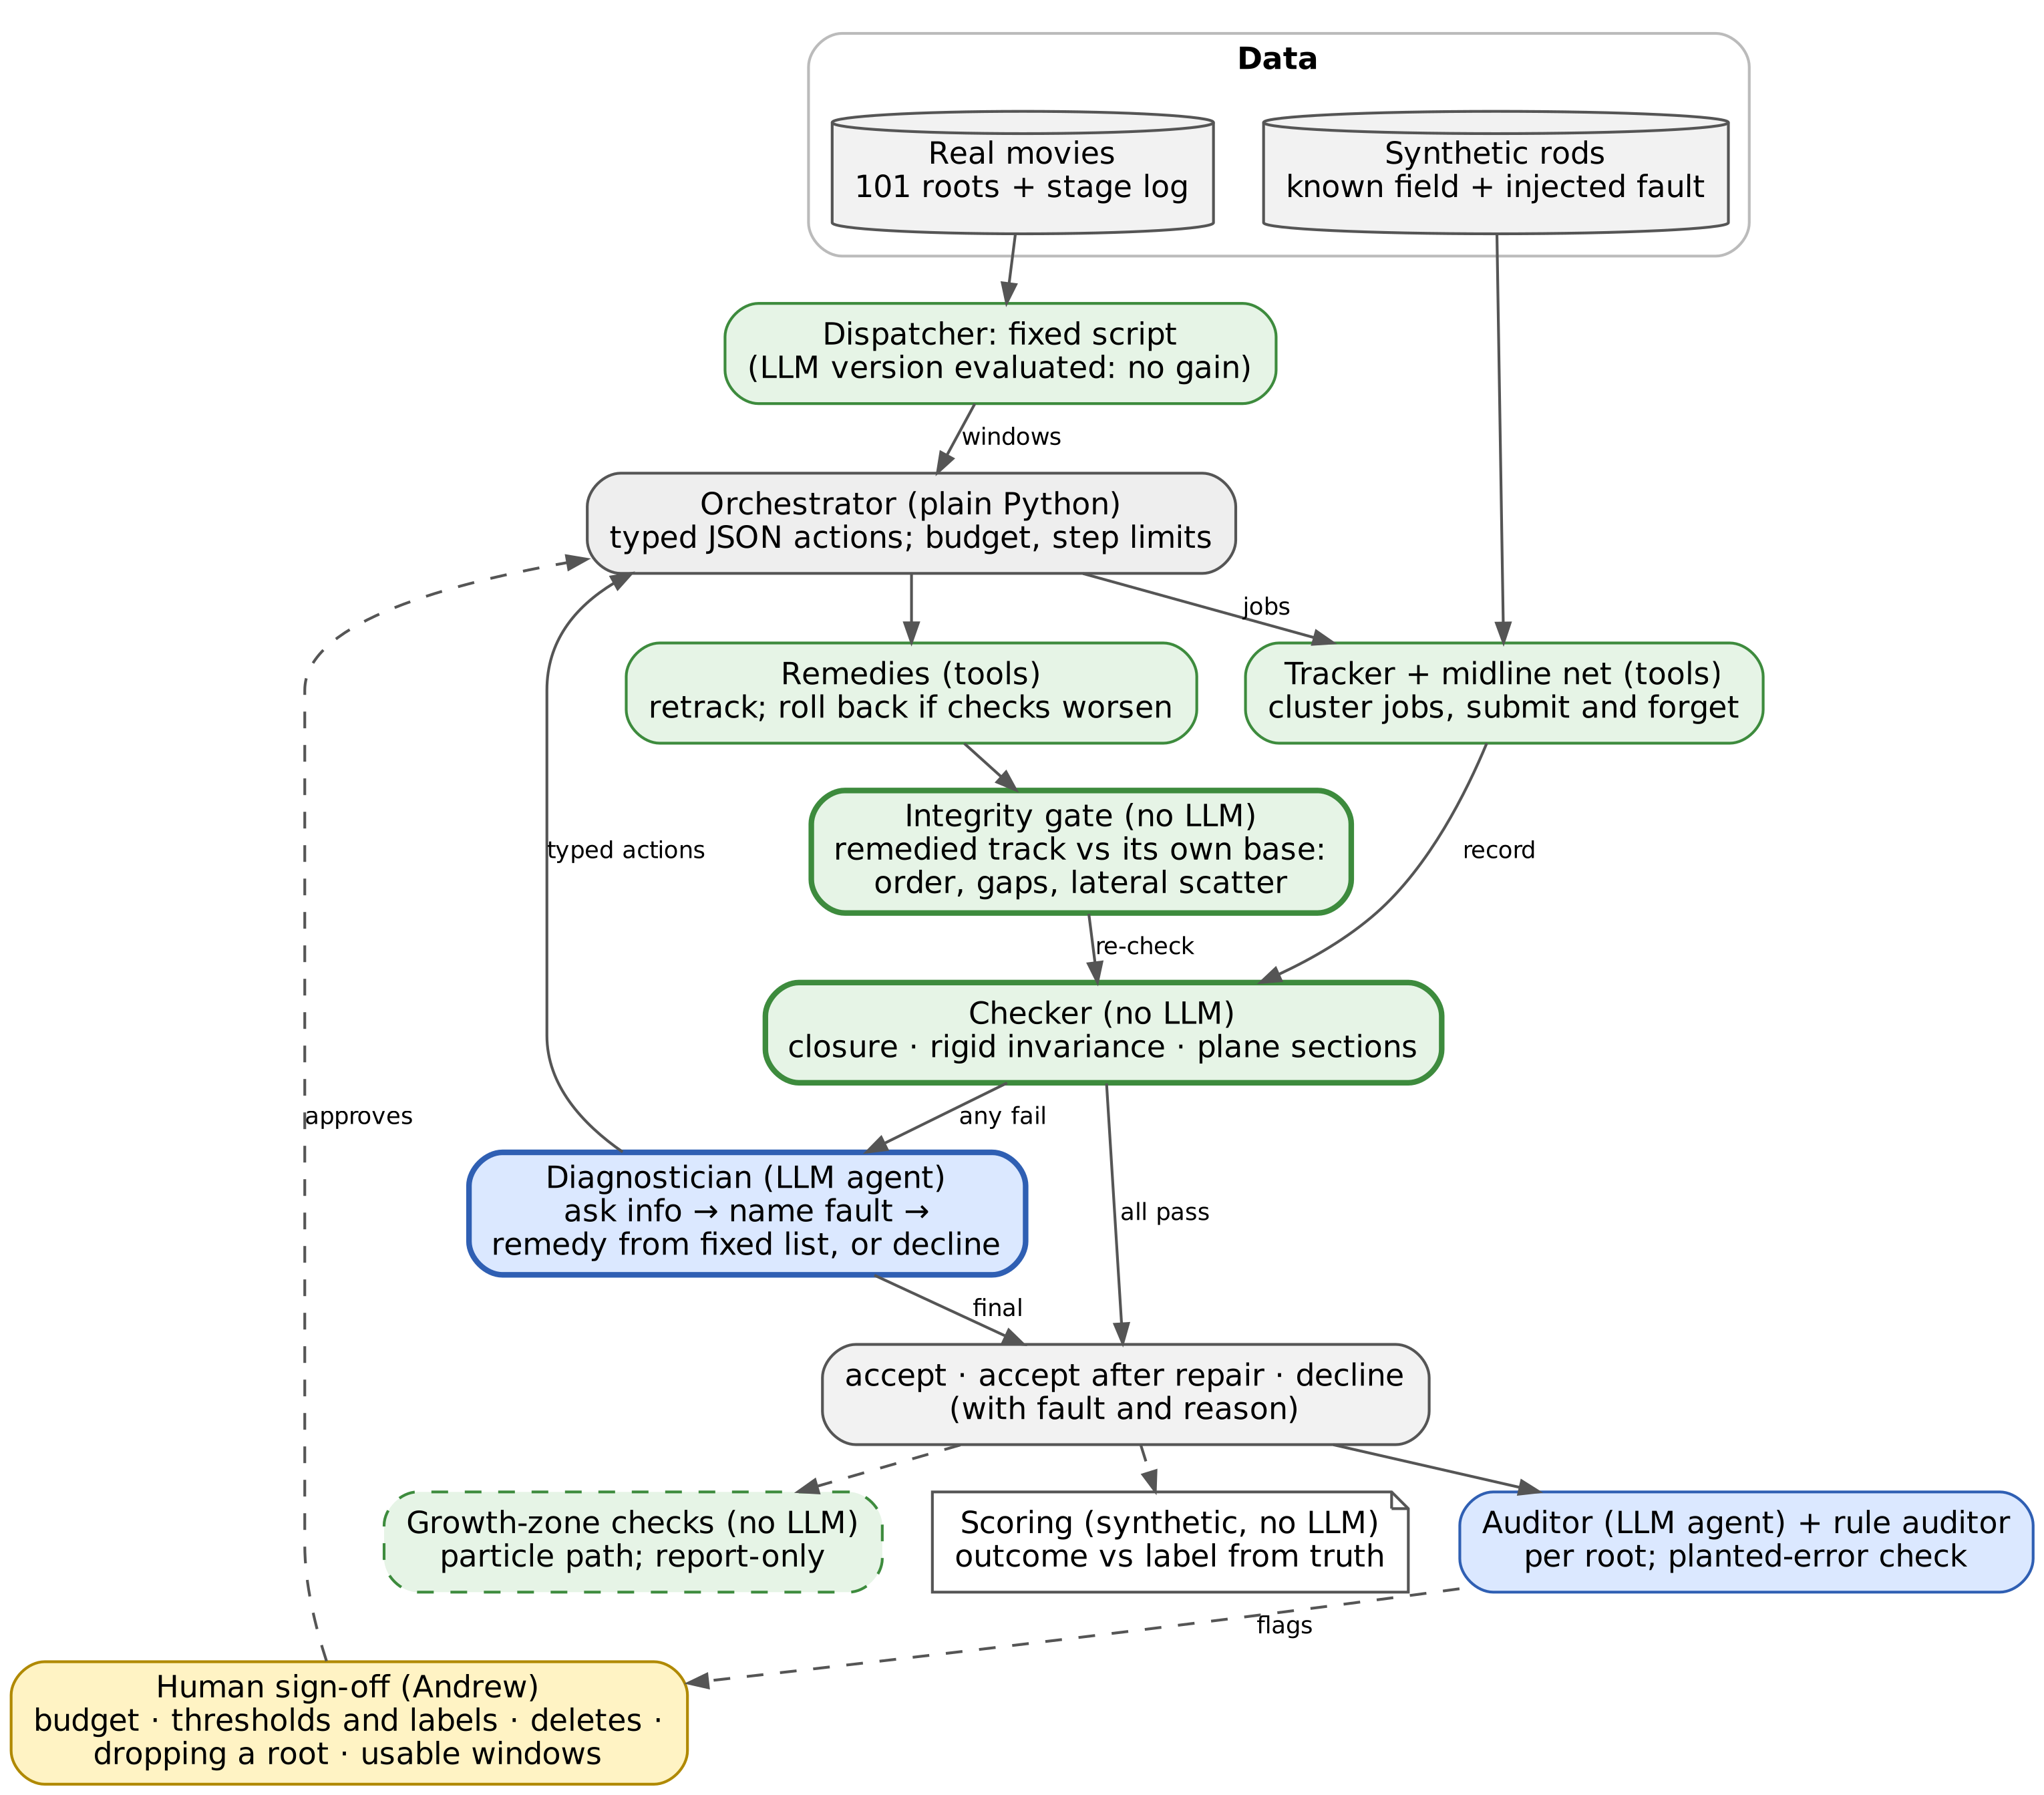
\includegraphics[width=0.78\textwidth]{fig_design.png}
\caption{Architecture. Blue: LLM agents. Green: deterministic tools (dashed: report-only). Grey: plain-Python orchestrator. Yellow: human sign-off. Every agent step is one typed JSON action, validated and executed by the orchestrator.}
\label{fig:design}
\end{figure*}

Fig.~\ref{fig:design} shows the system. A fixed-script dispatcher splits each root into two-hour windows inside the usable span set by the owner and submits tracking jobs to a computing cluster. The tracker (patch correlation on a midline from a trained network) returns a measurement record per window: tracked points along the midline and its two flanks for every frame, and the stage log.

\textbf{Checker (no LLM).} Three checks follow from kinematics. \emph{Closure}: integrated over the window, the tracked tip displacement in world coordinates must equal the stage-corrected displacement of the tracked chain,
\begin{equation}
C=\frac{1}{T}\Bigl\|\sum_t \bigl[\Delta\mathbf{x}^{\mathrm{w}}_{\mathrm{tip}}-\Delta(\mathbf{c}_0-\mathbf{c}_b)\bigr]\Bigr\|,
\end{equation}
with $T$ the window length, $\mathbf{c}_0$ the first and $\mathbf{c}_b$ the most basal tracked point. \emph{Rigid invariance}: a copy of the movie moved rigidly must give the same profile. \emph{Plane sections}: under Euler--Bernoulli kinematics the flank strain rates satisfy $\dot\varepsilon_+-\dot\varepsilon_-=-2h\,\dot\kappa$, with $2h$ the flank spacing and $\dot\kappa$ the curvature rate. Synthetic thresholds were set from the equations and clean rods (closure 1.0~px/h); on real movies closure gates at 19~px/h, the 95th percentile of 41 control windows, and the other checks are reported because most windows lack a moved copy.

\textbf{Diagnostician (LLM agent).} When a check fails, the agent may request evidence (stage-log residuals, velocity profile, frame quality, midline jitter, displacement relative to the patch radius), apply one remedy from a fixed list (frame registration, larger patch, changed frame stride, light midline smoothing, crop or mask of a second root, width-free ratio), accept, or decline with a named fault. After each remedy the measurement is retracked and rechecked; a remedy that worsens the checks is rolled back. The step limit is 8.

\textbf{Integrity gate (no LLM).} Closure is a sum and cannot see point order. After a registration remedy passed closure (22.8 to 14.0~px/h) on a track whose points were scrambled (neighbour gaps 1--166~px), every remedied track is compared with its own base track: point-order inversions, largest over median neighbour gap, and lateral scatter must stay within a factor $k$ of the base values, else the remedy is rolled back.

\textbf{Auditor (LLM agent) and rule auditor.} Once all windows of a root are final, the auditor reviews the accepted windows and flags outliers and inconsistencies; a rule auditor checks the same batch against fixed bounds.

\textbf{Human oversight.} The owner approves compute budgets, every threshold, label, prompt or remedy-list change after a scored run starts, any change to usable windows, dropping a root, and any delete. The model ID (\texttt{claude-opus-5-5}) and the client version are pinned; each agent step is one non-interactive call returning one schema-checked action.

\section{Evaluation Design}
\textbf{Synthetic rods.} Rendered rods with a prescribed velocity field, injected faults and fixed seeds give ground truth. Each rod is labelled \emph{accept\_clean}, \emph{accept\_repaired} or \emph{decline} by a tracker-only sweep over the base settings and every remedy, scored against the true field; labels, prompts, thresholds and seeds are committed before any method runs. Three sets were scored: freeze v4 (51 rods on unseen seeds: 18 clean, 9 repairable, 24 decline), and two held-out sets of compound and novel faults the remedy tree was not written for (c029: 24 rods, 20 labelled decline; c029b: 20 rods, 4/10/6, selected by a rule fixed before labelling because declining everything scored 20 of 24 on c029).

\textbf{Baselines.} A fixed script reports every measurement whose checks pass and declines the rest without remedies; a rule-based remedy tree applies a fixed fault-to-remedy sequence with the same tools; a single agent has the same model, actions and step limit but sees no checker output and has no roll-back. LLM methods ran three repeats.

\textbf{Metrics.} Balanced accuracy over the label classes; false accepts (a decline-labelled rod reported); agreement across repeats (Fleiss $\kappa$). On real windows there is no ground truth: an outcome is \emph{accepted after repair} if the checks pass after a kept remedy.

\section{Results}
\begin{table}[t]
\caption{Synthetic rods: balanced accuracy and false accepts per repeat}
\label{tab:synth}
\centering
\setlength{\tabcolsep}{3.5pt}
\begin{tabular}{lcccccc}
\toprule
 & \multicolumn{2}{c}{Freeze v4} & \multicolumn{2}{c}{c029} & \multicolumn{2}{c}{c029b} \\
Method & BA & FA & BA & FA & BA & FA \\
\midrule
Fixed script & 0.67 & 18 & 0.00 & 20 & 0.40 & 12 \\
Remedy tree & 0.93 & 2 & 0.70 & 4 & 0.77 & 4 \\
Diagnostician & 0.93 & 0 & 0.47 & 0.7 & 0.60 & 4.0 \\
Single agent & 0.63 & 0.3 & 0.06 & 5.3 & 0.43 & 6.3 \\
Decline all & 0.33 & 0 & 0.50 & 0 & 0.33 & 0 \\
\bottomrule
\end{tabular}
\end{table}

\textbf{Known faults.} On freeze v4 the diagnostician and the tree reached balanced accuracy 0.93 (diagnostician range 0.92--0.94 over repeats); the diagnostician made no false accept, the tree 2 and the script 18 (Table~\ref{tab:synth}). Without checker output the same model fell to 0.63, with 66 of 153 runs at the step limit. The diagnostician was consistent: 46 of 51 rods unanimous over three repeats ($\kappa=0.887$).

\textbf{Unseen faults.} On both held-out sets the tree was more accurate (overall 0.83 vs 0.72 on c029, 0.75 vs 0.48 on c029b). Most of the diagnostician's errors were declines of repairable rods (18 of 30 runs on accept\_repaired rods in c029b), typically after concluding that no listed fault explained the failed check; on c029 it made fewer false accepts than the tree (0.7 vs 4 per repeat). One fault kind (a mild second root with occlusion) defeated every method.

\begin{table}[t]
\caption{Integrated run on real windows (101 roots, 1,189 windows)}
\label{tab:real}
\centering
\setlength{\tabcolsep}{2.6pt}
\begin{tabular}{lcccccc}
\toprule
Method & Acc. & Repaired & Rule & Check & Agent/tree & Paused \\
\midrule
Integrated & 1034 & 2 & 58 & -- & 85 & 4 \\
Remedy tree & 1034 & 12 & 58 & -- & 78 & 7 \\
Fixed script & 1034 & 0 & 58 & 93 & -- & 4 \\
\bottomrule
\end{tabular}
\end{table}

\textbf{Real windows.} The integrated run (Table~\ref{tab:real}) covered every included root unattended over three nights on cached and cluster-retracked tracks, using 1,015 LLM calls and \$8.25 of a \$15 compute budget. 87\,\% of windows passed the checks unremedied and were reported by every method; 58 were declined by rule because closure could not be computed; the diagnostician ended 6 at the step limit, and 4 windows had no usable track. On the 90 failing windows both methods finished, they agreed on 74. A fresh run of one root from raw images reproduced the cached outcome in 12 of 12 windows.

\textbf{Auditor check.} In 30 batches of accepted synthetic windows, errors were planted in 15 (closure relabelled as passed, a track from another rod, velocities in the wrong unit, a doubled frame). The LLM auditor caught 9, 8 and 9 of 15 over three repeats and none of the wrong-unit plants; the rule auditor caught 15 of 15 but raised 55 false alarms on 225 clean runs against 20--25 for the LLM. Both are kept.

\textbf{Growth-zone placement.} Closure cannot see where along the root growth sits. A particle-path check integrates $\mathrm{d}X/\mathrm{d}t=v(X)$ from the measured profile and compares predicted with tracked positions. With thresholds from 150 real windows labelled by the owner (99.5th percentile of the 130 clean ones times 1.5), the shape check caught profiles shifted by 90~px (about 76~\textmu m) in 78\,\% of clean real windows with no false alarm, but almost no shift of 30~px or less (Fig.~\ref{fig:zone}). It is report-only.

\begin{figure}[t]
\centering
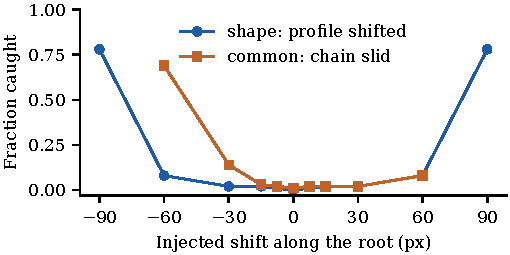
\includegraphics[width=\columnwidth]{fig_zone.pdf}
\caption{Growth-zone check on 130 clean real windows: fraction flagged when the measured profile is shifted along the root (shape part) or the whole tracked chain is slid (common part). At zero shift, 0 and 1 of 130 are flagged.}
\label{fig:zone}
\end{figure}

\textbf{Dispatcher.} An LLM dispatcher scheduled jobs on a simulated queue no better than a fixed script (equal or 0.5~h slower over five scenarios) and was removed from the loop.

\section{Reliability, Limitations and Safety}
The deterministic checks carried most of the reliability: they decide 87\,\% of real windows alone, and removing checker output cost the agent 0.30 in balanced accuracy. The agent's value was caution (no false accepts on known faults), not repair skill: on unseen faults a fixed rule tree repaired more. Two verifiers were added only after failures were observed (the integrity gate, the planted-error audit), which argues for designing checks of each remedy and each reviewer before trusting them. Labels on synthetic rods come from tracker-only sweeps; on real windows ``repaired'' means only that the checks pass. Closure is the only gate on real windows, and the zone check catches only gross misplacement. The system acts only through fixed tools; it cannot change thresholds, delete data or exceed the budget, and its LLM calls ran under a cap that was raised once mid-run (900 to 1,300, disclosed). An independent read-only audit of the whole project by a separate model session found 62 issues, none in a results table; real-root biology values found in the public history were masked and the history rewritten.

\section{Reproducibility}
The repository holds the code, a pinned model ID, \texttt{requirements.txt} and \texttt{environment.yml}, 509 offline tests, every proposal committed before its run, and one folder per result with its commands, tables and traces. Raw movies and the tracker are private; every table can be recomputed from committed outputs, and the offline demo runs without them.\footnote{\url{https://github.com/AndrewOldag/oldag_andrew_me295_project_repo}}

\section{Conclusion}
A checker-guided agent can make the repair-or-decline call on known faults as accurately as a rule tree and with fewer false accepts, but it does not generalize its repairs to faults outside its list. For high-throughput growth kinematics the practical design is deterministic checks first, a rule tree for known repairs, and an agent where caution matters more than coverage. Next steps are the 24~h strain-rate maps the system was built for, a gating version of the zone check, and per-fault analysis of the agent's unnecessary declines.

\bibliographystyle{IEEEtran}
\bibliography{refs}

\appendix
\section*{AI Use Declaration}
\begin{itemize}
\item \textbf{Claude Code (Opus 5.5), build sessions:} nearly all code, tests, runs and results READMEs, from specs approved by the author. Checked by 509 deterministic tests, proposals and labels committed before runs, an independent audit, and the author's review of each session's log and results; the code was not read line by line by the author.
\item \textbf{Claude (Opus 5.5), planning account:} specs, design review, merges, drafts of the lab reports, the figures and this paper. The author approved each decision and edited the text.
\item \textbf{Claude Code (Fable 5.2), audit session:} read-only audit of the project (62 findings); each finding was checked against the evidence before a fix was accepted by the author.
\item \textbf{Gemini 4 Argon:} read-only audit of the freeze v4 metrics (recomputed with independent code, no disagreement).
\item \textbf{Claude Science:} literature network used for related work; digests audited blind.
\item \textbf{\texttt{claude-opus-5-5} inside the system:} the diagnostician, auditor, dispatcher and single-agent baseline under test; their outputs are scored by code against labels and planted errors.
\end{itemize}
The author designed the research question and evaluation, set usable windows, hand-labelled the reference windows for the zone check, reviewed the checker, scoring and metrics code against the equations, and approved every threshold and budget.

\end{document}
